\section{System Design}\label{sec:system_design}
\begin{figure}[h]
\centering
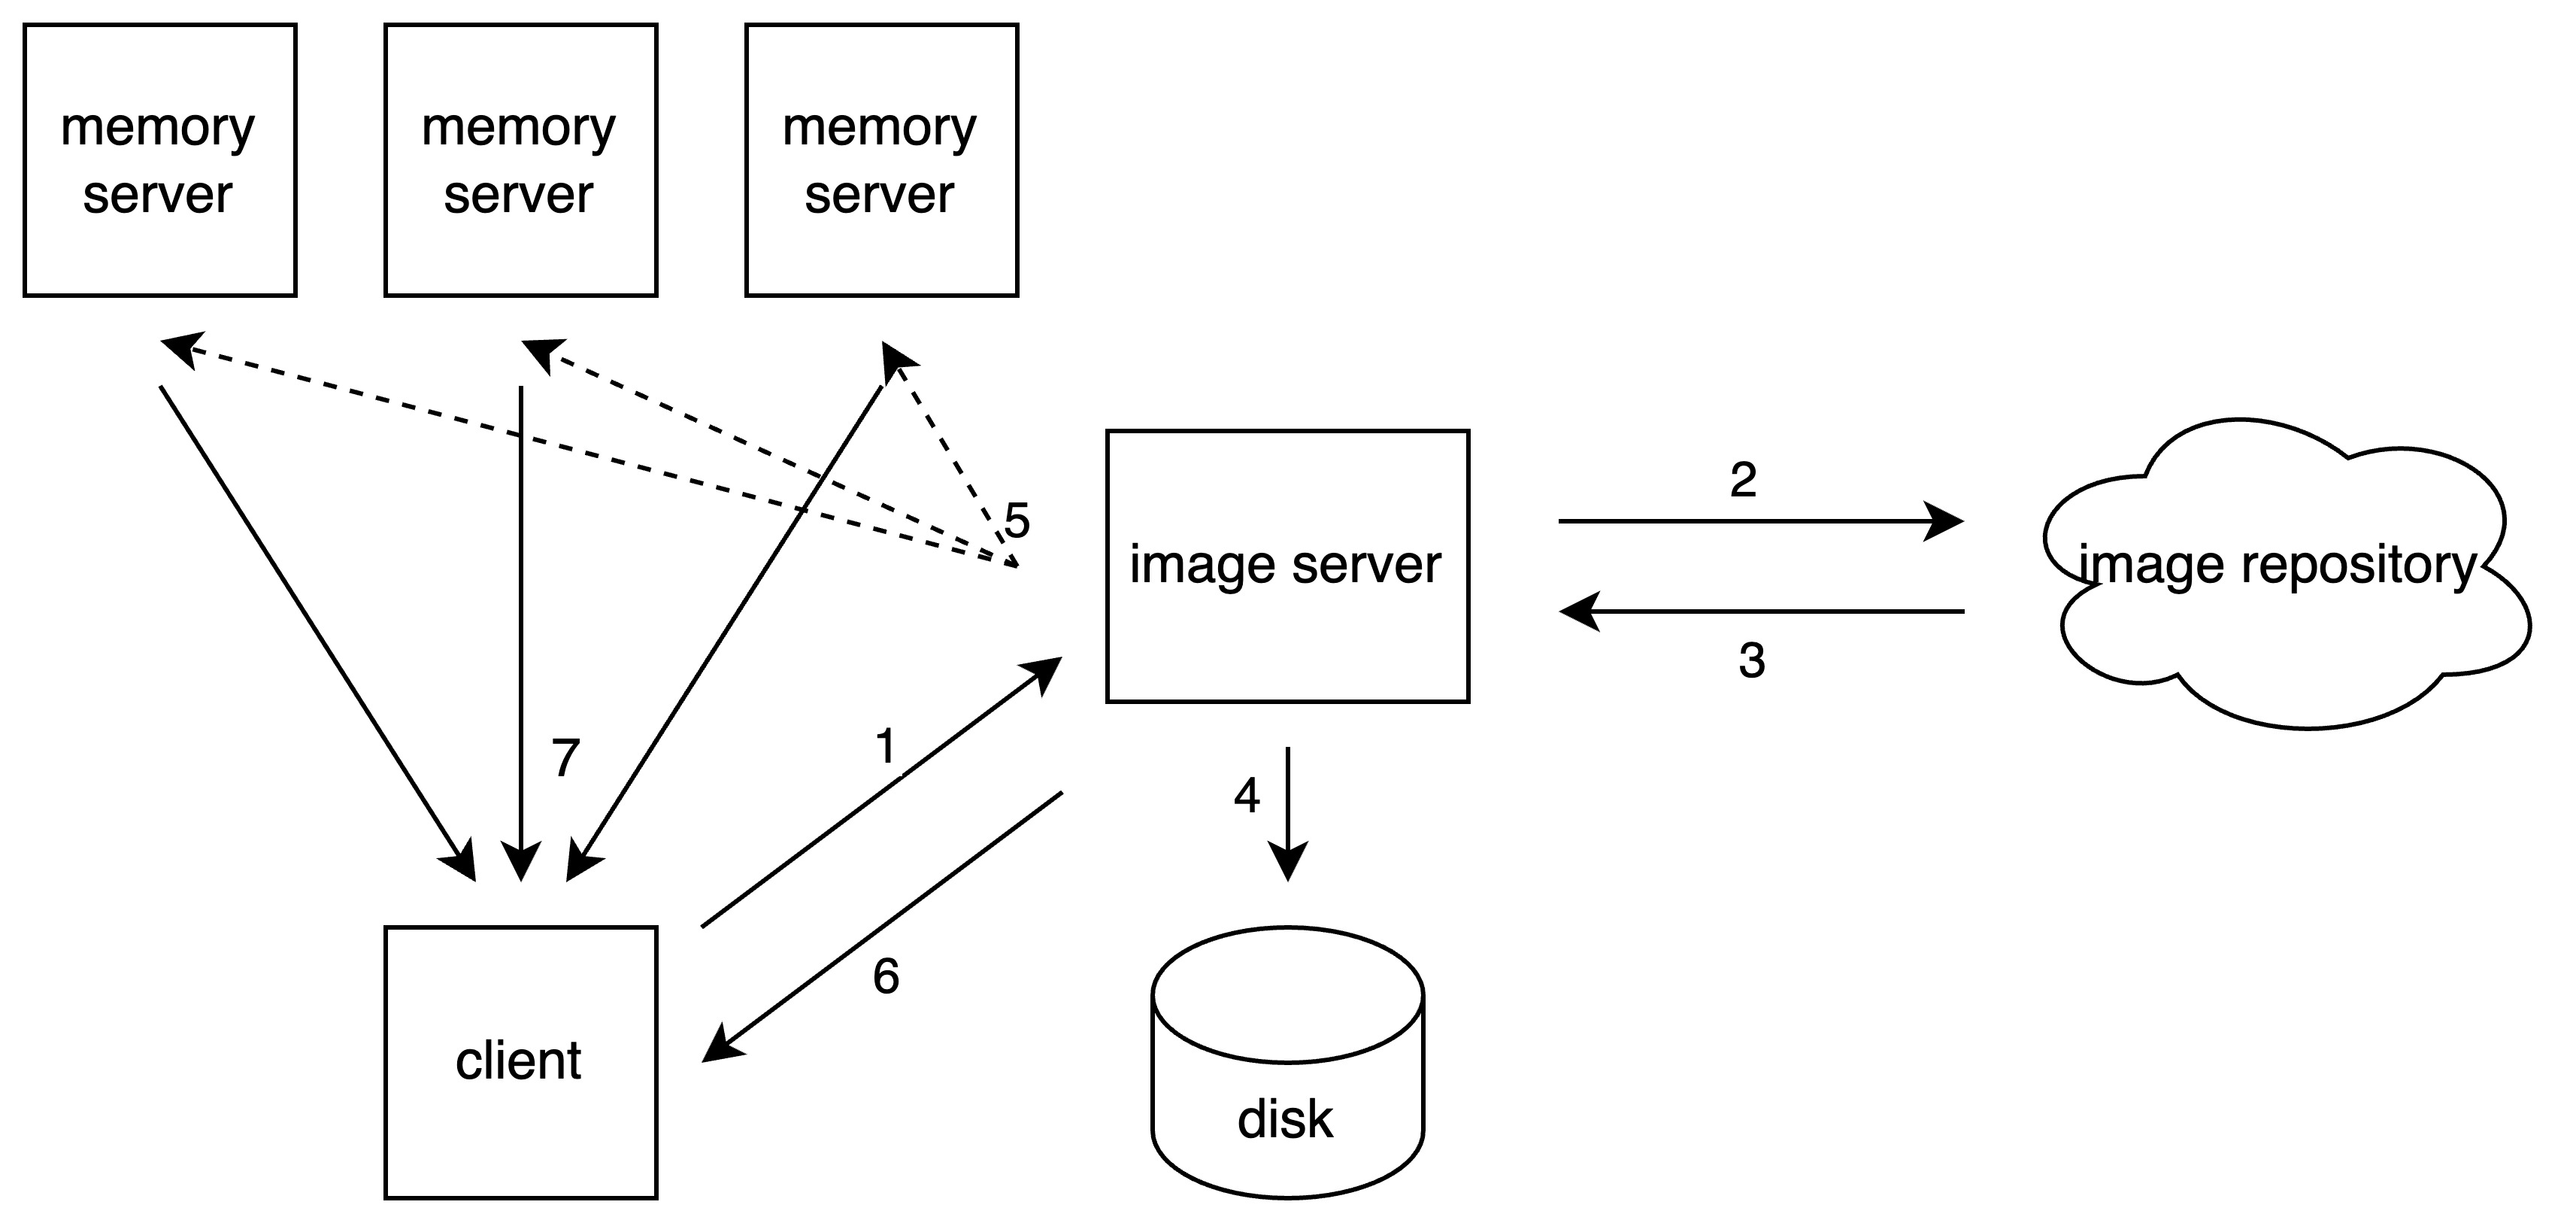
\includegraphics[width=0.45\textwidth]{flow.jpg}
\caption{ImageHarbour system architecture}
\label{fig:imageharbour_architecture}
\end{figure}
ImageHarbour is designed as a distributed image caching system that leverages stranded memory resources across multiple hosts in a data center. The system architecture consists of three main components: the image server, the memory servers, and the client nodes. Figure \ref{fig:imageharbour_architecture} provides an overview of the ImageHarbour system design. The client flow to fetch an image is as follows: Clients contact the image server to fetch a new image (step 1). The image server checks if the image is in the cache, if the image is not in the cache, it fetches the image from an image repository (steps 2-3) and stores it locally on disk (step 4). Additionally, the image server splits the image into fixed size chunks and stores the chunks on the memory servers using one-sided RDMA operations (step 5). The image server then returns a metadata response, containing the location of the chunks in the memory pool to the client (step 6). The client finally performs one-sided RDMA read operations to fetch the image data directly from the memory servers (step 7). If the image is already cached, steps 2-5 are skipped. Additionally, the clients can cache the metadata of the image to avoid contacting the image server for future requests (as opposed to caching the entire image) thereby skipping steps 1-6 for subsequent requests.

\subparagraph*{\textbf{Image Server}}
The image server is the client interface to ImageHarbour. It makes intelligent caching decisions, coordinates the allocation and deallocation of memory resources, and maintains metadata about the cached images. The image server performs the following functions:

\noindent\textit{Metadata Store.} The image server maintains information about the cached images, including their unique identifiers, sizes, access frequencies, and locations within the memory pool.

\noindent\textit{Caching Engine.} The image server decides which images should be cached in the memory pool and which images should be evicted when the cache reaches its capacity. It can employ algorithms, such as Least Recently Used (LRU) or Adaptive Replacement Cache (ARC) \cite{megiddo2003arc}, to make caching decisions based on factors like image popularity and access patterns.

\noindent\textit{Memory Allocator.} The image server manages the allocation and deallocation of memory resources within the memory pool. It keeps track of the available memory on each host and assigns memory regions to cached images based on their sizes and access frequencies.

\subparagraph{\textbf{Memory Servers}}
Memory servers act as passive storage nodes that provide memory resources to the memory pool managed by the image server. Each memory server registers with the image server and the image server distributes the cached images across the available memory servers. All operations to the memory servers (apart from the initial setup) are one-sided RDMA operations that do not interrupt the CPU on the memory server. 

\subparagraph{\textbf{Client Nodes}}
Client nodes are the consumers of the cached Docker images. They interact with ImageHarbour to retrieve images from the memory pool instead of fetching them from disk or over the network.

\subparagraph{\textbf{Scalability}}
ImageHarbour is designed to scale horizontally by adding more hosts to the memory pool as the demand for cached images grows. The control plane dynamically manages the distribution of images across the memory pool hosts to achieve load balancing.